%!TEX root = ../report.tex
\chapter{Evaluation}

\textit{Peer-to-peer systems are distributed systems consisting of interconnected nodes able to self- organize into network topologies with the purpose of sharing resources such as content, CPU cycles, storage and bandwidth, capable of adapting to failures and accommodating transient populations of nodes while maintaining acceptable connectivity and performance, without requiring the intermediation or support of a global centralized server or authority.} -- Androutsellis and al.~\cite{Androutsellis-Theotokis:2004}.

%\section{Decentralization}

%TBD: Qualitative evaluation of the level of decentralization of all sub-systems.

%\section{Resilience}

%TBD: Qualitative evaluation of crashes and attacks, according to the trust model, that the network might experience and the result of %experiments that simulate their occurrence.

The majority of the time spent in the project concerned the deployment of the libraries on the lab machines in the School of Computer Science department at McGill University. A number of challenges had to be overcome to obtain a working setup. However, unresolved issues in the libraries prevented scaling the system to a number high enough to perform more interesting analyses of the empirical behaviour of the system. This chapter therefore explains the issues that had to be solved to obtain a working setup, the remaining issues that prevent scaling to a higher number of nodes and present preliminary empirical results that were obtained on a small network.

\section{Deployment issues and solutions}

Under the umbrella of deployment issues are included some that are specific to the libraries, such as compilation issues in building the libraries from source code, since no pre-compiled libraries are currently available, some that are specific to the lab configuration at McGill University, such as the automatic suspension of unused machines, and some that result from the incompatibility between the development and deployment environments used by the MaidSafe developers and those that were available at McGill. The intention here is to draw attention to implicit issues that arise in trying to use the libraries to inform potential users of their nature and help the developers resolve them in the future.

To avoid introducing errors in the deployment tests, one of the \textit{routing\_node} example executable, which is a basic interpreter built by the MaidSafe developers using their libraries, was used without modification to make sure that all deployment issues would be resolved before introducing additional problems due to a different usage of the API than what has been tested. Most of all solved issues were handled by a custom python script that controlled the behaviour of the \textit{routing\_node} process by supplying commands through the standard input and parsed the standard output of commands to retrieve the relevant information.

\subsection{Unreliable uptime of lab machines at McGill}

Lab machines are suspended to conserve energy when not in use. They cannot be resumed from network activity, so a physical interaction is required to resume them. Since the tests were performed over WiFi from a different building than the one which hosts the machines, it was impractical to go physically interact with the machines to wake them up. 

Tests were therefore performed on the set of up machines, which could even be changing hour to hour. The initialization of the system therefore probed all the lab machines every two hour to assess which were up and available and stored the list on disk for subsequent runs of the script.

\subsection{Lack of control of the execution environment of the nodes}

Lab machines could and were used for other concurrent tasks by other users during the tests, so it was impossible to control the resource usage of the machines, making any kind of load analysis inaccurate. Performance tests therefore measured latency of communication because these were lightly affected by lightweight concurrent tasks (web browsing, etc.) performed by other users, which seemed to compromise most of the external load that was observed.

\subsection{Mismatch between the development environment of the libraries at MaidSafe and the deployment environment at McGill}

The developers chose to use the latest features of recent C++ compilers, that are part of the upcoming C++11 standard. That support is incomplete and buggy in the most recent versions of GCC, leading to wasted time in debugging compilation issues. Fortunately, the Clang compiler provides adequate support for them. However, the 32-bit 12.04 Ubuntu images in the labs do not have installed packages that provided recent versions of the Clang compiler tool chain and no root access is possible to fix the installations.

The problem was resolved by using a VirtualBox Virtual Machine running Ubuntu 13.04 32-bit to compile the libraries and \textit{routing\_node} executable. Once compiled these could be deployed and used on the lab machines.

However, recent updates to the source code in the last weeks required recent features of standard C libraries (glibc), which are not present on the older lab images. That last problem was not resolved because the location of the library expected by the executable is fixed at compile time by the build system. Two solutions are possible. Either the library on the deployment machines could be upgraded, which is not possible without root access and moreover, being a core library of a linux image, risk completely breaking its configuration, or the build options of the MaidSafe executable would need to be changed, which was not possible given the default options and would therefore have required a deeper understanding of the internals of the build system. 

A previous version of the source code, dating from October 10th was therefore used, even if it exhibited problems explained later, which at the time of writing, may or may not be solved by a more recent version.

\subsection{Deployment of modified binaries}

Once compiled on a dedicated local virtual machine, the binaries needed to be deployed to the lab machines. Since modifications of the source code were few in the tests I performed, it was not worth automating and the executable was copied using shell commands. 

Fortunately, the lab machines use a user partition that is hosted on a Network File System share, which means that once the executable was copied to the home directory, it was available from any of the lab machines. 

\subsection{Control of a distributed network}

Starting and connecting every node of the network, and controlling their operations while the system is running is non-trivial with more than two nodes, especially in the presence of failures. After different experiments with scripting languages, Python was chosen because it provides, Paramiko, a really useful library that abstract the communication over an SSH channel. However, once the node is running and being controlled from the script, it was difficult to connect to manually interact with it to diagnose problems in the network.  The linux \textit{screen} utility was used to interact with nodes in a separate process from the one used to start the node over ssh. Shutdown of the node was done by killing the screen processes. 

Some nodes required more control from the script than simply being started and stopped, for bootstrapping the network and obtaining the routing tables of the other nodes. In this case, direct interaction was done over SSH by the script with no possibility of concurrent manual inspection and interaction. Sending commands was done by writing to the standard input of the node process and parsing the standard output with regular expressions. Since the Paramiko only provides synchronous communication primitives, careful timing of standard output reading from the script was required to avoid blocking on yet to be sent outputs.

\subsection{Placement of logical nodes on physical machines}

At first, experiments were done by having a single logical node on each physical machine. Uniformity in the delay of transmission of messages (every message is a local network request-reply) and guaranteed true concurrency in the execution of the different nodes to avoid multi-tasking and task scheduling between the nodes (which nonetheless still happens with the other processes) made the performance analysis easier. The performance evaluation of Section~\ref{sec:Performance} was done with that setup and further details are provided later.

However, routing of messages issues were discovered that required more nodes to be created than the number of physical machines available and therefore required refactoring the script to support multiple logical nodes on a single physical machine. The number of concurrent ssh connections that could be supported by a single python interpreter became an issue (the maximum number of thread that could be created was around 370) and therefore, one SSH connection per machine was done to initialize multiple nodes using the \textit{screen} utility.

As a side note, a latency analysis in the presence of non-uniform connections between nodes is more complicated since communication through a socket between processes on the same machine is significantly faster than from a local network message exchange. Preliminary tests for small messages (64 bytes) at the overlay layer, showed a 50\% latency increase of LAN messages compared to messages exchanged between processes on the same machine (11 ms vs 6 ms).

\subsection{Propagation of the changes in the network}

When run from a script, the initialization commands for the different nodes, and the experiment operations were executed too fast for the system to have time to setup and stabilize.  An artificial delay of 10 seconds was introduced to give time to routing tables to stabilize and information to propagate. That delay was chosen given the official documentation statement that churn event could be seen by the network most of the time within 6 seconds of happening.

\subsection{Debugging of crashes and performance issues}

This is a fundamental problem in a distributed system, especially if the problems result from many interactions between multiple nodes. Since most of the problems were observed right after initialization once the first commands were sent, more complicated issues did not really manifest. When that happens, some logging infrastructure (such as the Linux Trace Toolkit) would be necessary.

The influence of the number of hops was investigated by obtaining the routing tables of each node on a small network and computing the number of hops of the shortest path between every pair of nodes. The graphs of the next section were generated by ordering the results according to their latency and number of hops and aggregating the latency results for nodes at a similar distance.

\subsection{Non-determinism in the configuration of the overlay routing tables}

Although the identifiers of the nodes, which are used to partition the distributed hash table among the available nodes, were fixed and the nodes were always started in the same order with the same identifiers, the content of the routing tables of each node changed slightly from execution to execution, even in the absence of failure because the routing tables are partly greedily populated from message that go through the nodes. The initial dissemination of the first messages is non-deterministic and therefore influence the content of the routing tables.

That prevented determining the topology of the overlay network once for a given configuration in the absence of failure. Therefore, it needed to be determined each time the network was restarted, which happens for every set of experiments.

\subsection{Unresolved issues}

Once the network was up and running, tests with a small number of nodes, up to 30 nodes on different machines, were successful most of the times. However, increasing the number of nodes, or running more nodes on the same machine, exhibited issues that could not easily be resolved.

Sometimes, a message would traverse more than 50 hops, which because of assertions in the source code, would crash the node on which the assertion is performed. This happened when requesting the routing table of all the nodes from a single node, preventing the initial topology of the overlay network to be determined reliably.

Other times, some nodes would fail to provide their routing tables on the first request but would then provide it later on. 

Other times, especially when multiple nodes would run on the same physical machine, the RUDP connection would be lost with one of the nodes.

Finally, sometimes, communication with a particular node would fail although communication with and from an intermediary node would succeed, breaking the transitive connectivity property of the network.

In all the cases, the debugging tools that were available and the understanding of the inner workings were insufficient to efficiently debug what was going on. Interaction on the development mailing list, although generally insightful, failed to capture enough information about the running system to allow the developers to easily provide sufficient solutions to the problems mentioned.

\section{Performance}
\label{sec:Performance}

%TBD: For all metrics, an abstract analysis in function of the number of nodes in the network is performed, knowing the behaviour of the underlying Novinet primitives, to assess scaling. In addition, an empirical statistical analysis is performed.

\subsection{Experimental setup}

\subsubsection{Physical topology}

Figure~\ref{fig:PhysicalTopology} illustrates the connections between the lab machines used for the experiments. The latency introduced by the routers is negligible. Tests performed using the \textit{ping} utility between machines behind the same router and behind different routers showed no clear latency penalty by going through an extra hop. All measures of round-trip delay were under 1 millisecond for 64 byte packet, around 1 ms for 1008 bytes packets ,and around 2.5ms for 10008 bytes packets with no clear indication that an extra hop introduces a significant delay. Therefore, for all purposes we can assume that lab machines are fully connected to one another with channels of similar latency.

\begin{figure}[htb]
\begin{center}
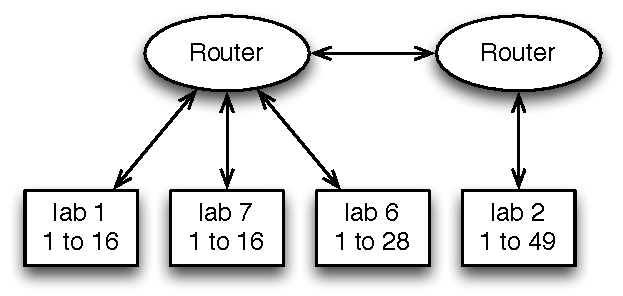
\includegraphics[width=0.5\textwidth]{figures/PhysicalTopology}
\caption[Physical topology]{\label{fig:PhysicalTopology} Physical topology of McGill's School of Computer Science lab machines used for experiments, as determined using \textit{tracepath} utility. Machines behind the same router only see one communication hop between each other. Machines behind different routers see two hops. However, experiments with the \textit{ping} utility indicate that the extra hop does not affect latency significantly, therefore under a light load we can consider all machines to have similar connectivity to their neighbours.}
\end{center}
\end{figure}

\subsubsection{Machine configurations}
There is great variability in the configuration of the different machines, with a mix of older and newer processor models and different amount of installed RAM, with some machines having as much as 16 GB of RAM available while others have 2 GB. Some examples of machine configuration are shown in Table~\ref{tb:MachineConfigurations}.

\begin{table}[htdp]
\begin{center}
\begin{tabular}{|l|c|}
\hline
Machine & Lab 1-4 and 1-5 \\
\hline
Processor & Intel Core 2 Quad CPU    Q8200  @ 2.33GHz\\
\hline
Cache Size & 2048 KB\\
\hline
RAM Size & 4 GB\\
\hline
Network Speed & 100Mb/s\\
\hline
\end{tabular}
\end{center}

\begin{center}
\begin{tabular}{|l|c|}
\hline
Machine & Lab 2-1 and 2-3 \\
\hline
Processor & Intel Core 2 Duo CPU     E8135  @ 2.40GHz\\
\hline
Cache Size & 6144 KB\\
\hline
RAM Size & 2 GB\\
\hline
Network Speed & 100Mb/s\\
\hline
\end{tabular}
\end{center}
 
 \begin{center}
\begin{tabular}{|l|c|}
\hline
Machine & Lab 2-2  \\
\hline
Processor &  Intel Core i7-3770S CPU @ 3.10GHz\\
\hline
Cache Size & 8192 KB\\
\hline
RAM Size & 16 GB\\
\hline
Network Speed & 100Mb/s\\
\hline
\end{tabular}
\end{center}
 
\begin{center}
\begin{tabular}{|l|c|}
\hline
Machine & Lab 6-8 \\
\hline
Processor &  Intel Core i5 CPU         650  @ 3.20GHz\\
\hline
Cache Size & 4096 KB\\
\hline
RAM Size & 4 GB\\
\hline
Network Speed & 100Mb/s\\
\hline
\end{tabular}
\end{center}

\begin{center}
\begin{tabular}{|l|c|}
\hline
Machine & Lab 7-14 \\
\hline
Processor &  Intel Core 2 Duo CPU     E7600  @ 3.06GHz\\
\hline
Cache Size & 3072 KB\\
\hline
RAM Size & 3.8 GB\\
\hline
Network Speed & 100Mb/s\\
\hline
\end{tabular}
\end{center}

\caption[Example machine configurations.]{Example machine configurations. There are many different generations of processors and widely different amount of RAM, but all machines use the same Ubuntu linux 12.04.3 LTS 32-bit image.}
\label{tb:MachineConfigurations}
\end{table}%

 
 All the machines run the same Ubuntu linux 12.04.3 LTS 32-bit image even though they could support 64-bit operating system and applications. This is probably done to simplify administration of the machines as there might be some old 32-bit machines still being used in the department.

The heterogeneity might not affect the results significantly since the 32-bit operating system image probably targets the common denominator among the different machines, in terms of instruction support, and the operations of the MaidSafe libraries are probably well within the memory limitations of even the least powerful machine.

\subsubsection{Operating system setup}

The load on the machines could not be controlled since they could be used at any time by students while the experiments were running. However, it is probably reasonable to assume that the load on the machines was light in general and since experiments could be performed in a matter of minutes, the load was probably stable throughout the experiment.

\subsubsection{Overlay configuration}
\label{sec:OverlayConfiguration}

The MaidSafe-Routing library maintains an overlay network on top of the IP network between the physical machines. Each node has a routing table with information about other nodes of the network, up to a fixed number of nodes, defined when the application was compiled. The default settings reserve 64 entries in the routing table for other nodes. However, this number is almost equivalent to the number of concurrently running physical machines in the labs, which means that each node could directly talk with any other node. The intended use case of the library is to connect millions of nodes over the internet, which would make it unrealistic to have each node know about any other node. To simulate limited connectivity between nodes on a smaller network, the maximum number of entries in the routing table was set to 8 instead of 64 and the closest nodes size was set to 2 instead of 8 (from a suggestion on the mailing list)~\footnote{Communication on the mailing list indicates that the distribution of the hashing algorithm can be significantly altered by changing the number of entries in the routing tables, which can lead to false results. For the purpose of our application, where the overlay network is only used to establish secure communication channels between nodes, a bad distribution of entries might make some paths between nodes longer. Since our tests specifically take into account the number of hops in the network that is not an issue. See \url{https://groups.google.com/d/msg/maidsafe-development/EN6bTek_TpY/zBZ_es2_PGsJ}}. The closest nodes parameter controls the number of neighbours for which a node will maintain extra information, in addition to their ID, to improve the accuracy of determining which nodes are closest to a given key. For the purpose of this evaluation, it can be considered an optimization parameter. Figure~\ref{fig:OverlayTopology} illustrates a fictive example with 6 nodes and a maximum number of entries of 3 in routing tables. Notice that every node is at a maximum distance of 2 hops from any other node. Some nodes, such as 1 and 4, can have less than the maximum number of entries in their routing table.

\begin{figure}[htb]
\begin{center}
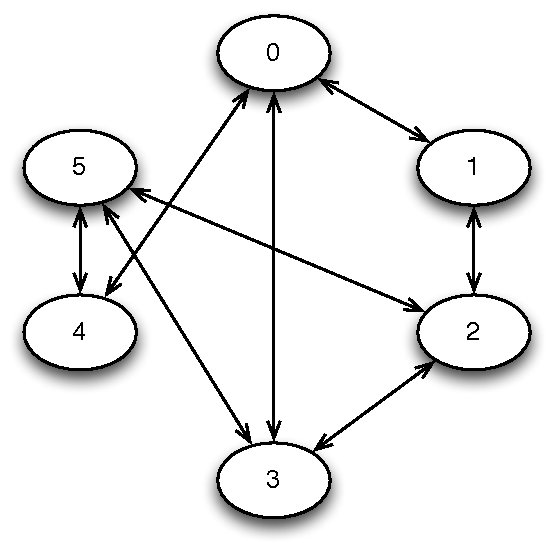
\includegraphics[width=0.4\textwidth]{figures/OverlayTopology}
\caption[Overlay topology fictive example.]{\label{fig:OverlayTopology} Overlay topology fictive example. Nodes have a maximum number of 3 entries in their routing tables. Some nodes, such as 1 and 4, might have less than 3 entries. In this particular example, every node is at a maximum distance of 2 hops from one another.}
\end{center}
\end{figure}

The performance evaluation was done using the \textit{routing\_node} test application~\footnote{Using commit $84985d5e40a0a8c3049e18868cec790f1e408aef$ of the MaidSafe super-project from October 10th}, which is part of the MaidSafe-Routing library. It should provides results representative of the performance that could be expected from the McChat application because it adds very little functionalities that might impact the performance of the application on top of the core libraries: the core feature is simply to send text messages between users, that are associated with nodes. 

\subsubsection{Controlling experiments}

All experiments are automatically setup and performed using a python script running on a single machine that controls all nodes from individual ssh connections. It means that executing commands on a node generates network traffic between the node's machine and the control script's machine (which usually runs on the same machine as one of the nodes). For latency testing, it should have little effect. However, for throughput or load testing it might mean that the observer effect is sufficiently significant to influence the results. This could be mitigated by having every node run a local script that would run a predefined set of commands according to some external time to remove communication overhead. Since I only did latency experiments, the complexity of the setup was not deemed worthy of the effort. Figure~\ref{fig:ExperimentControl} illustrates the current control mechanism for experiments.

\begin{figure}[htb]
\begin{center}
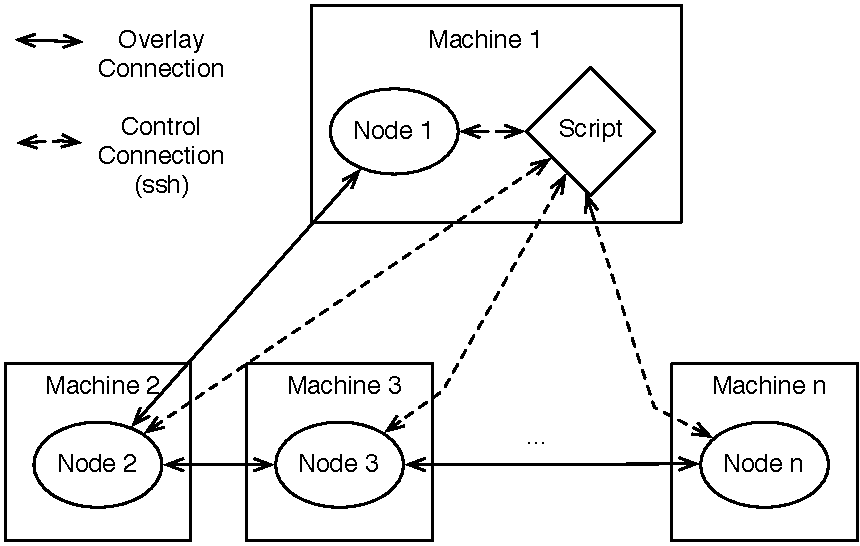
\includegraphics[width=0.6\textwidth]{figures/ExperimentControl}
\caption[Experiment Control.]{\label{fig:ExperimentControl} Experiment Control. A python script executing on one of the node machine control every node of the network  through ssh connections. Every command sent to nodes therefore generates network traffic both for sending the command and receiving the results. For small messages, the length of the output result of the node can therefore be higher than the message itself, potentially leading to higher network traffic caused by the control connections than the overlay network.                                                                                                                                                                                                                                                                                               }
\end{center}
\end{figure}

\subsection{Latency of message send}

\subsubsection{Comparison between the latency of TCP and MaidSafe overlay networks}

The MaidSafe platform provides pseudo-connected, end-to-end encryption of message exchanges and NAT-traversal, in a fully-decentralized peer-to-peer fashion. This section quantifies the latency overhead of providing such guarantees using their approach, compared to using the TCP protocol over IP layer (connection-oriented but not-encrypted).

The latency of packets was performed between the \textit{lab2-1} and \textit{lab1-4} machines on the local network. The TCP latency was measured using the \textit{netperf}~\footnote{\url{http://www.netperf.org/netperf/}} utility using the following options:
\begin{verbatim} netperf -H lab1-4 -t TCP_RR -v 2 -- -r <size>,1 \end{verbatim}
which starts an experiment between \textit{lab2-1} and the a net server running on \textit{lab1-4}, by doing a TCP request response experiment sending a packet of size $<size>$ and a 1-byte response. The \textit{-v 2} option simply, activate the verbose output mode to print the round-trip latency.

Latency on the MaidSafe network was measured using two nodes on the same machines, directly connected to one another, using the \textit{senddirect} command of their \textit{routing\_node} utility and setting the size of the packet with the \textit{datasize} command.

Results and their interpretation are given in Table~\ref{tb:LatencyMaidSafeVsTCP} and the relative latency ratio are illustrated in Figure~\ref{fig:LatencyMaidSafeVsTCP}. The results indicate an overhead between 21x and 28x and would suggest that the overhead grows as the size of the packet increases. Note however that these latency figures were obtained on a local area network while the intended use case for the MaidSafe platform is on a wide area network. Since the major latency increase comes from the encryption of the communication and is independent of the physical transmission of the message, the ratio on a wide area network would be lower.

\begin{table}[htdp]
\begin{center}
\begin{tabular}{|l|r|r|r|}
\hline
Packet size & TCP latency (ms) & Overlay latency (ms) & Ratio \\
\hline
32 &  0.5 & 11 & 22\\
\hline
1024 & 0.57 & 12 & 21\\
\hline
32768 & 3.5 & 85 & 24\\
\hline
1048576 & 90.6 & 2518 & 28\\
\hline
\end{tabular}
\end{center}
\caption[Absolute and relative latency increase of MaidSafe RUDP compared to TCP]{Absolute and relative latency increase of MaidSafe RUDP compared to TCP. The latency 
measurements for packet sizes of 32 and 1024 is similar in both cases, the decrease in the ratio is due to a proportionally larger increase in time for TCP packets (.57ms vs 0.5 ms) compared to MaidSafe RUDP packets (12 ms vs 11 ms) which might be caused by the rounding of values to the nearest ms by MaidSafe tool. The similar absolute latency times for packets of size 32 and 1024 is probably caused by the usage of a single IP packet in both cases. For larger packets, both absolute and relative latency time increase as the packet size is bigger, probably caused by a longer processing time of the packet value or additional validation messages during the communication.}
\label{tb:LatencyMaidSafeVsTCP}
\end{table}%


\begin{figure}[htb]
\begin{center}
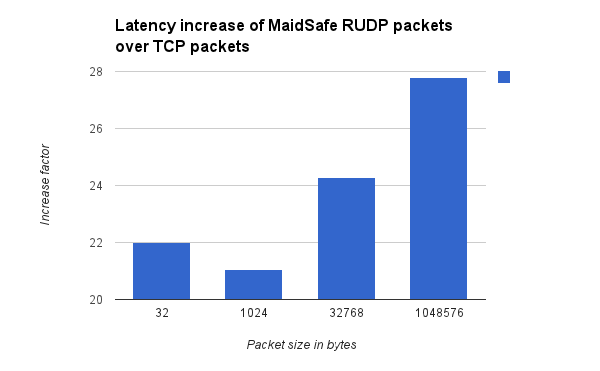
\includegraphics[width=0.8\textwidth]{figures/LatencyMaidSafeVsTCP}
\caption[Relative latency increase of MaidSafe RUDP compared to TCP]{\label{fig:LatencyMaidSafeVsTCP} 
Illustrated relative latency increase of MaidSafe RUDP compared to TCP on a local area network between two nodes directly connected to one another.                                                                                                                                                                                                                                                                                                }
\end{center}
\end{figure}


\subsubsection{Influence of the number of hops}

The determining factor in the latency of messages in the network seems to be the number of hops between nodes, i.e. the number of intermediary nodes on the shortest path between the sender and the receiver node. Experiments were performed on a 15 nodes network with defaults parameters except for the number of entries in the routing table that was changed from 64 to 8, which controls the number of neighbours a node keeps connection to, and the number of closest nodes that was changed from 8 to 2~(which is an optimization parameter, as explained in the previous "Overlay configuration" section. These changes were suggested to allow simulation of the behaviour of a larger network with a smaller number of nodes~\footnote{\url{https://groups.google.com/d/msg/maidsafe-development/EN6bTek_TpY/zBZ_es2_PGsJ}}. Each node was running on a different machine.

The latency between pairs of node, from a single node to all the nodes was measured and sorted in order of average latency over 10 experiments for different message lengths. Figure~\ref{fig:LatencyPerReceiver} compares the results for three different message sizes, 32, 1024 and 16384 bytes, the first two were chosen because they illustrate independence from the message size up to a certain limit and the last because it was the biggest value that was tested. Although the order of the nodes in the sorting varies slightly according to the different sizes, they all show strikingly similar patterns, with results clustered in three groups that closely correspond to the number of hops between the nodes. Notably, in each group two nodes seem to be faster than the others, which might be caused by the closest node optimization parameter~\footnote{However, different experiments with the same parameters, although they provided similar patterns of latency, had a differing number of faster nodes per group, so no clear conclusion could be drawn about their link to the closest nodes parameter.} Additionally, the increase in latency is between a factor of 2 and 3 when the message is small but gets bigger as the message increases.



\begin{figure}
\begin{center}
\begin{minipage}[b]{.5\textwidth}
\begin{center}
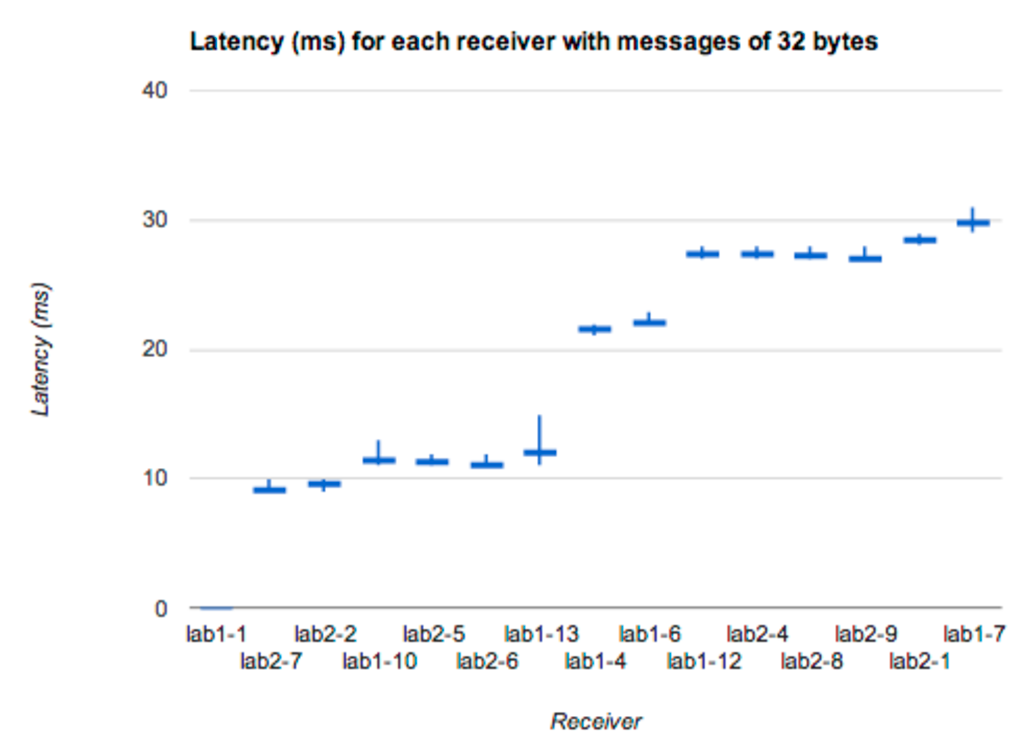
\includegraphics[width=\textwidth]{figures/LatencyPerReceiver-32b}
\end{center}
\subcaption{32 bytes}\label{fig:LatencyPerReceiver-32b}
\end{minipage}%
\begin{minipage}[b]{.5\textwidth}
\begin{center}
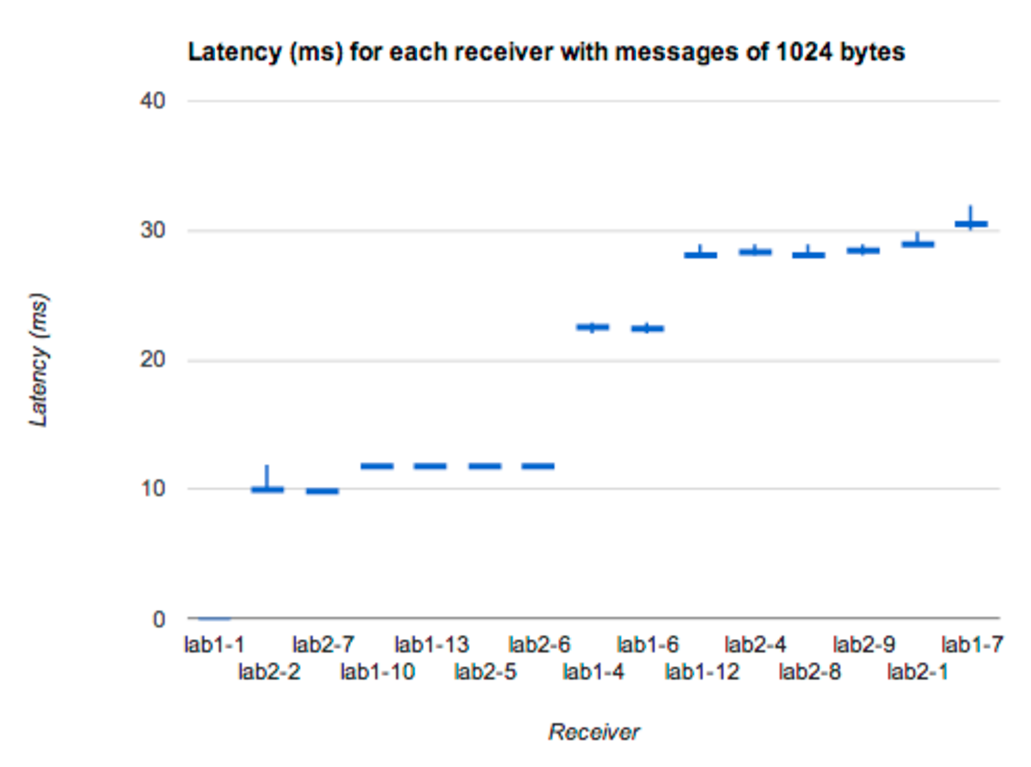
\includegraphics[width=\textwidth]{figures/LatencyPerReceiver-1024b}
\end{center}
\subcaption{1024 bytes}\label{fig:LatencyPerReceiver-1024b}
\end{minipage}
\hfill
\begin{minipage}[b]{\textwidth}
\begin{center}
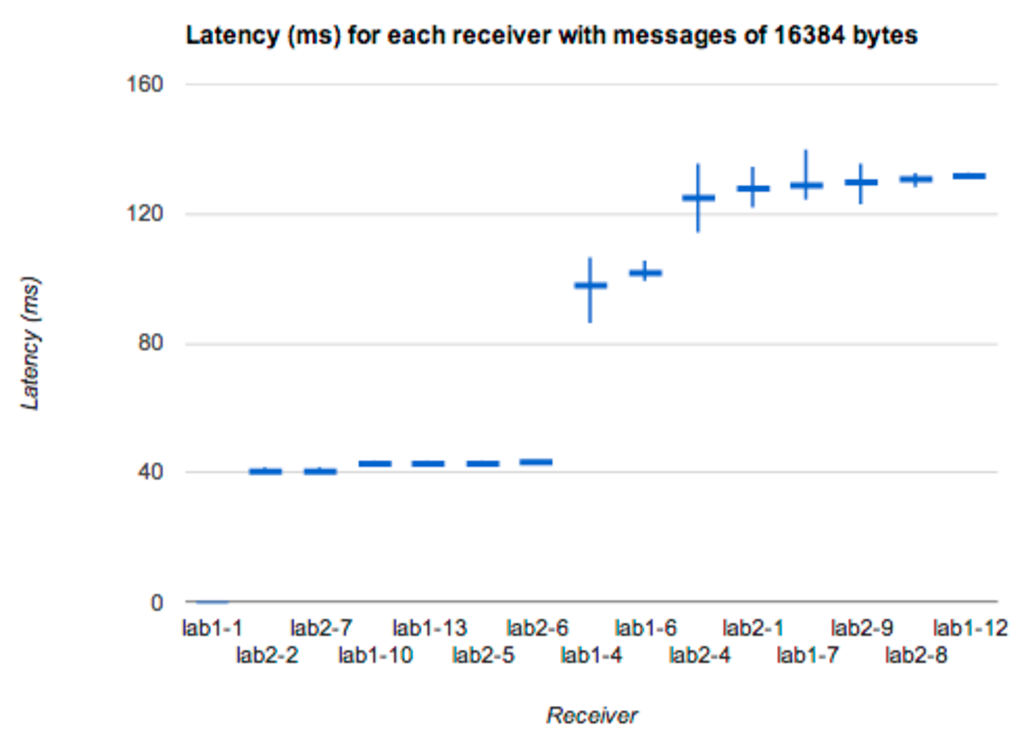
\includegraphics[width=.5\textwidth]{figures/LatencyPerReceiver-16384b}
\end{center}
\subcaption{16384 bytes}\label{fig:LatencyPerReceiver-16384b}
\end{minipage}
\caption[Pairwise latency (ms) from a single node in a 15 nodes network.]{Pairwise latency (ms) from \textit{lab1-1} node to all other nodes in a 15 nodes network for different message sizes. Horizontal bar shows average and vertical bar shows range between the minimal and maximal values taken from 10 measurements. Results cluster in 3 different groups that corresponds to the number of hops between the sender and receiver. Latency for 0 hops, when lab1-1 sends the message to itself is under 1 millisecond and reported as 0ms. The next six values shows the latency for nodes 1 hop away. The other values shows results for nodes 2 hops away.}\label{fig:LatencyPerReceiver}
\end{center}
\end{figure}

Comparison in latency for increasing hops, as the message size grows is illustrated in Figure~\ref{fig:LatencyComparisonsHopsMsgSize}. Up to sizes of 4096 bytes, latency results are mostly independent of the message size. Since latency is mostly determined by encryption time, 4096-bytes is likely the element chunk size that is used for encryption (this size varies according to network fragmentation). For bigger messages, the latency time is at least the sum of the time to encrypt all the message chunks. As shown on the graph, latency grows faster than linearly with the number of hops and that growth increases with the size of the message but the exact source of that additional latency has not been identified yet. 


\begin{figure}[htb]
\begin{center}
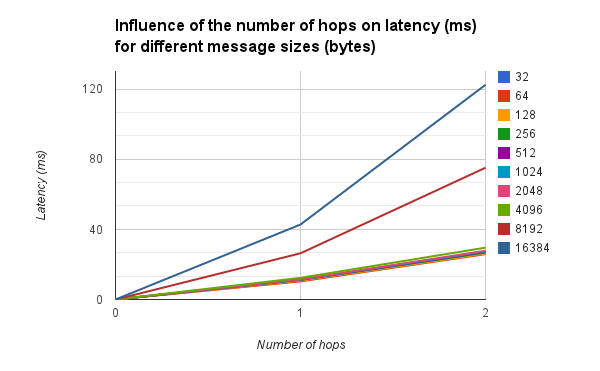
\includegraphics[width=0.8\textwidth]{figures/LatencyComparisonsHopsMsgSize}
\caption[Influence of the number of hops and message size on latency.]{\label{fig:LatencyComparisonsHopsMsgSize} Influence of the number of hops and message size on latency. Each line shows the average value of all nodes at a given distance in hops for a given message size on a 15 nodes network. The same results as for Figure~\ref{fig:LatencyPerReceiver} are used, with additional message sizes. Interestingly, up to 4096 bytes, latency results are similar and directly proportional to the number of hops. Since latency is dominated by the encryption time, it suggest that the basic chunk size of encryption is at most 4096-bytes. For bigger messages, latency for two hops is more than twice than that of 1 hops and the ratio is growing bigger with the size of the message. The additional source of latency has yet to be identified.
}
\end{center}
\end{figure}


%\subsection{Latency for joining the network}

%\subsection{Overhead of maintaining the routing tables}

%\subsection{Speed of reconfiguration of the network}